\documentclass[10pt]{article}
\usepackage{graphicx, fancyhdr, enumerate}
\usepackage{amsmath, amsfonts, color, multicol, mathtools}
\usepackage{blkarray}

\setlength{\topmargin}{-.55 in} 
\setlength{\textheight}{9 in}
\setlength{\textwidth}{6.625 in} 
\setlength{\evensidemargin}{-.0625 in}
\setlength{\oddsidemargin}{-.0625 in} 
\setlength{\parindent}{0 in}
\setlength{\headheight}{18.0pt}
\newcommand{\ds}{\displaystyle}
\newcommand{\xbar}{\overline{X}}

\DeclarePairedDelimiter{\ceil}{\lceil}{\rceil}

\cfoot{\thepage} 
\renewcommand{\headrulewidth}{0.4pt} 
\renewcommand{\footrulewidth}{0pt} 
\newcommand{\ansfont}[1]{{\textcolor{blue}{\textbf{Answer:}}\ \ #1}}


\lhead{\Large\sffamily Stat 330 (Fall 2016): Homework 2} 
\rhead{\sffamily Due: September 7, 2016}

% Uncomment the following line to remove answers, and comment line out to show answers:
\renewcommand{\ansfont}[1]{}


\begin{document}
\pagestyle{fancy} 
Show all of your work, and \emph{please} staple your assignment if you use more than one sheet. Write your name, the course number and the section on every sheet. 

\begin{enumerate} 
  \item A certain lottery consists of a bucket of white balls numbered 1 through 69 and a bucket of red balls numbered 1 through 26. In a drawing, 5 white balls are randomly selected without replacement and 1 red ball is randomly selected. You buy one ticket consisting of 5 white numbers and 1 red number:
    \begin{enumerate}
      \item How many possible drawings are there? i.e., determine $|\Omega|$.
			\item Let $A$ be the event that your ticket matches all the white numbers drawn (order does not matter) and the red number. Find $P(A)$ (Leave as a fraction).
			\item Let $B$ be the event that your ticket matches all the white numbers drawn (order does not matter) but not the red number. Find $P(B)$ (Leave as a fraction).
			
    \end{enumerate}
    \ansfont{
		\begin{enumerate}
      \item There are $69\choose5$ ways to drawn 5 balls out of the 69 white balls without replacement. For each of these combinations, there can be 26 red balls to go with it. Using the multiplication principle, there are $69\choose5$ $\cdot$ 26 = 292,201,338 possible drawing combinations.
			\item There is $5\choose5$ = 1 way to match the 5 white numbers and $1\choose1$ = 1 way to match the red number. So, $|A|$ = $1 \cdot 1 = 1$ and $P(A) = \frac{1}{292201338}$
			\item There is $5\choose5$ = 1 way to match the 5 white numbers and $25\choose1$ = 25 ways to match the non-drawn red ball. So, $|B|$ = $1 \cdot 25 = 25$ and $P(B) = \frac{25}{292201338}$
			\end{enumerate}
    }



  \item Suppose that there are 15 entries in an art contest.
    \begin{enumerate}
      \item If cash prizes of different amounts are awarded for first, second, and third place, how many different ways can these prizes be awarded?
      \item If, instead of cash prizes, the contest gives ribbons to the top three entries, without distinguishing between first, second, and third place, how many different ways can these prizes be awarded? 
      \item Suppose that three of the 15 entries belong to the same artist, named Megan. A lazy judge decides to award ribbons to three entries by randomly selecting three numbers between 1 and 15, without replacement. What is the probability that at least two of Megan's entries win ribbons?
    \end{enumerate}
    \ansfont{
    \begin{enumerate}
\item Since different prizes are awarded, order matters. There are $P(15,3)=2,730$ different ways to award the prizes.
\item Now order does not matter so there are $15\choose3$=455 different ways.
\item Let A=``Exactly 2 ribbons'' and P=``3 ribbons''. Then since A and B are disjoint, 
$P(A \cup B)=\frac{|A|}{|\Omega|}+\frac{|B|}{|\Omega|}.$ Then $|A|$=$3\choose2$ $12\choose1$, $|B|$=$3\choose3$ $12\choose0$, and $|\Omega|=455$. Thus $P(A \cup B)=\frac{36}{455}+\frac{1}{455}=\frac{37}{455}=0.0813$.
\end{enumerate}
     }
      %  \item Let A=``Exactly 2 ribbons'' and P=``3 ribbons''. Then since A and B are disjoint, $P(A\cup B)=\frac{|A|}{|\Omega|}+\frac{|B|}{|\Omega|}=\frac{3\choose2 12\choose1}{15\choose3}+\frac{3\choose3 12\choose0}{15\choose3}=\frac{36}{455}+\frac{1}{455}=\frac{37}{455}=0.0813$.

 \item
   Suppose license plates have 6 entries. The first three entries must be letters (A-Z), and the last three must be digits (0-9). \emph{Letters and digits can be used more than once.} A license plate is selected randomly. What is the probability that the letters O, I, and Z and the digits 0 and 1 were not used for this plate?\\
	
    \ansfont{
        The number of all possible plates $=|\Omega|=(26)^3 \cdot (10)^3$.  The number of plates excluding O, I, Z, 0, 1 $=|A|=(23)^3 \cdot (8)^3$. $P(\text{plate excludes O, I , Z, 0, 1}) =\frac{|A|}{|\Omega|}=\frac{(23)^3 \cdot (8)^3}{(26)^3 \cdot (10)^3}=(0.8846 \cdot 0.8)^3=0.3544$
    }

  \item The first three digits of a university phone exchange are 452. If all the sequences of the remaining four digits are equally likely, what is the probability that a randomly selected university phone number contains seven distinct digits? 
	
	\ansfont{
	$|\Omega|=10^4=10,000$. Let A = the event that the  4 digits are one of $\{0,1,3,6,7,8,9\}$. Then $|A|=  7\cdot 6 \cdot 5 \cdot 4$ or $P(7,4)$. Thus the required probability $=\frac{|A|}{|\Omega|}=\frac{840}{10000}=0.084$
	}
    
	\item A committee consists of five Caucasians, three Hispanics, two Asians, and two African-Americans.
A subcommittee of four is formed at random. 
		\begin{enumerate}
		\item What is the probability that all ethnic groups are represented in the subcommittee? 
		\item What is the probability of at least one non-Caucasian member being in the subcommittee? 
		\end{enumerate}
		
\ansfont{

Total possible subcommittees $\displaystyle =|\Omega|= \binom{12}{4}=\frac{9\cdot 10 \cdot 11 \cdot 12}{2  \cdot 3 \cdot 4}=495$.
        	\begin{enumerate}
		\item The number of subcommittees representing all ethnic groups $\displaystyle=|A|=\binom{5}{1}\binom{3}{1}\binom{2}{1}\binom{2}{1}=60$ so that $P(\text{all ethnic groups represented})=60/495=4/33=0.1212$
		\item $\displaystyle P(\text{at least 1 non-Caucasian member})=1-P(\text{0 non-Caucasian members})=\displaystyle 1-\frac{\binom{5}{4}}{\binom{12}{4}}=98/99$
		\end{enumerate}
}
			
    
    
\item Baron 2.14

\ansfont{

\begin{center}
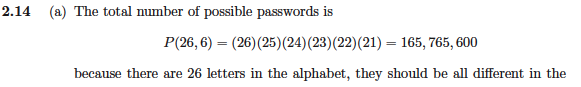
\includegraphics[width=0.9\textwidth]{baron2-14a}

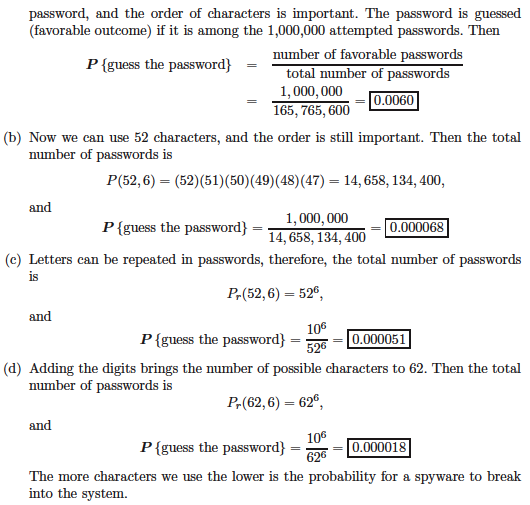
\includegraphics[width=0.9\textwidth]{baron2-14b}
\end{center}
}
\end{enumerate}
\end{document}
